\chapter{常用的python模块}
\section{Argparse}
argparse模块是一个用户用户友好的命令行接口,当用户每有给定可用的参数时,argaprser能自动生成帮助和使用信息。
\begin{python}
import argparse
parser = argparse.ArgumentParser(description='Process some integers.')
parser.add_argument('integers',metavar='N',type=int,nargs='+',help='an integer for the accumulator')
parser.add_argument('--sum',dest='accumulate',action='store_const',const=sum,default=max,help='sum the integers(default:find the max)')
args = parser.parse_args()
print(args.accumulate(args.integers))
\end{python}
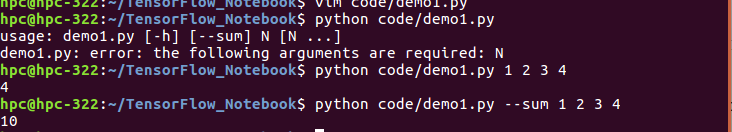
\includegraphics[scale=0.5]{demo1.png}\newline

代码能根据传入的参数选择相应的函数计算。
\begin{itemize}
\item 创建一个parser
\item 增加arguments
\item 解析参数
\end{itemize}

\subsection{ArgumentParser 对象}
class argparse.ArgumentParser(prog=None, usage=None, description=None, epilog=None, parents=[], formatter\_class=argparse.HelpFormatter, prefix\_chars='-', fromfile\_prefix\_chars=None, argument\_default=None, conflict\_handler='error', add\_help=True, allow\_abbrev=True)
\begin{itemize}
\item prog:程序的名字(默认为sys.argv[0])
\item usage:描述程序用法的字符串。(默认通过arguments增加到parser)
\item description:argument帮助前的文本展示。(默认为:None)
\item epilog:argument帮助之后的文本展示。(默认为:None)
\item parents:应该被包含的列表对象。
\item formatter\_class:自定义输出帮助的类。
\item prefix\_chars:参数前面的字符。(默认为'-')
\item fromfile\_prefix\_chars:应该被读的文件的字符串。
\item argument\_default:参数的全局值。(default:None)
\item conflict\_handler:解决冲突选项的策略。(通常不是必需的)
\item add\_help:增加-h/--help选项到parser。(默认为True)
\item allow\_abbrev:如果缩略不冲突,可以允许长的选项被缩略。(默认为True)
\end{itemize}
\subsection{prog}
默认情况下ArgumentParser对象用sys.argv[0]决定如何显示程序的名字。
\begin{python}
#filename:arg1.py
import argparse
parser = argparse.ArgumentParser()
parser.add_argument("echo")
args = parser.parse_args()
print(args.echo)
\end{python}
默认情况下ArgumentParser从包含用法信息的参数计算useage message。
\begin{python}
import argparse
parser = argparse.ArgumentParser()
parser.add_argument('--foo',help='foo help')
args = parser.parse_args()
\end{python}

\begin{figure}[htbp]
\centering
\subfigure[name of the subfigure]{
\begin{minipage}{5cm}
\centering

\includegraphics[scale=0.5]{demo2.png}
\end{minipage}}
\subfigure[name of the subfigure]{ 
\begin{minipage}{5cm}
\centering
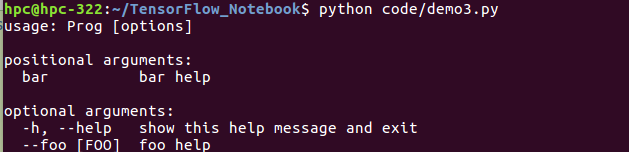
\includegraphics[scale=0.3]{demo3.png}
\end{minipage}}
\label{fig:1}
\end{figure}
大多数的ArgumentParser构造体用description=关键字,这个参数给出一个简单的程序说明其如何工作的。在帮助信息中表述在命令行和帮助信息之间。
\begin{python}
import argparse
parser = argparse.ArgumentParser(description='A foo that bars')
parser.print_help()
\end{python}
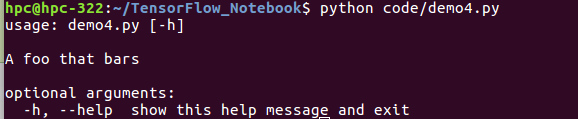
\includegraphics[scale=0.5]{demo4.png}\newline
一些程序喜欢在参数表述后添加一些额外的信息说明,这些说明可以通过ArgumentParser中的epilog=参数指定。
\begin{python}
import argparse
parser = argparse.ArgumentParser(description='A foo that bars',
epilog="And that's how you'd foo a bar")
parser.print_help()
\end{python}
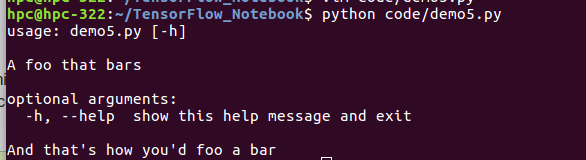
\includegraphics[scale=0.5]{demo5.png}\newline
有时候一些parser共享一些参数,相比于重复定义这些参数,一个单个的parser通过传递parents给ArgumentParser。parents=参数得到一个ArgumentParser对象的列表对象,从中收集所有的位置和选项行为\newline
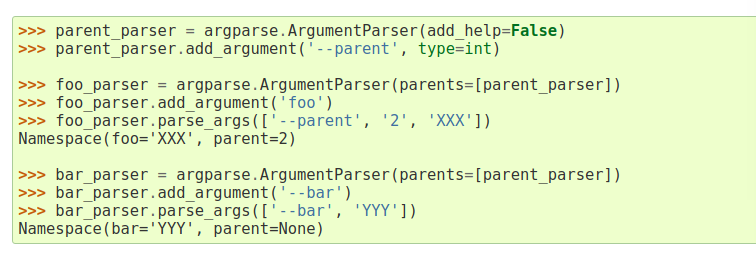
\includegraphics[scale=0.4]{demo6.png}\newline
大多数的parent parser指定add\_help=False,因此ArgumentParser将看到两个帮助选项(一个在parent一个在child)同时报错。你必须在通过parsers=传递前必须完全初始化parser,如果你在child parser改变parent parsers,改变将不被反映到child。
formatter\_class
ArgumentParserdurian允许指定可用的格式化类自定义格式,当前有4个类:
\begin{itemize}
\item argparse.RawDescriptionHelpFormatter
\item argparse.RawTextHelpFormatter
\item argparse.ArgumentDefaultHelpFormatter
\item argparse.MetavarTypeHelpFormatter
\end{itemize}

RawDescriptionHelpFormatter和RawTextHelpFormatter在如何显示说明上给与更多控制,默认ArgumentParser对description和epilog在命令终端一行显示。
\begin{python}
import argparse
parser = argparse.ArgumentParser(prog='PROG',description='''this
 description was indented wierd
but that is okey''',
epilog='''
likewise for this epilog whose whitespace will be
cleaned up and whose words will be wrapped
across a couple lines''')
parser.print_help()
\end{python}
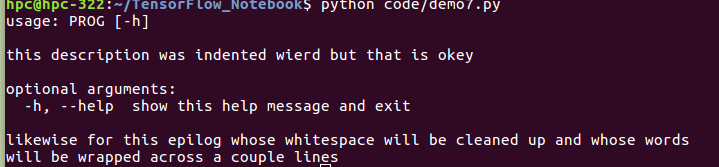
\includegraphics[scale=0.5]{demo7.png}\newline
传递RawDescriptionHelpFormatter作为formatter\_class=让description和epilog正确显示。
RawTextHelpFormatter主要维持素有的帮助文本,值描述的信息。\newline
ArgumentDefaultHelpFormatter:自动增加关于值的默认信息。\newline
\begin{python}
import argparse
parser = argparse.ArgumentParser(prog='Prog',
formatter_class = argparse.ArgumentDefaultsHelpFormatter)
parser.add_argument('--foo',type=int,default=42,help='FOO')
parser.add_argument('bar',nargs='*',default=[1,2,3],help='BAR!')
parser.print_help()
\end{python}
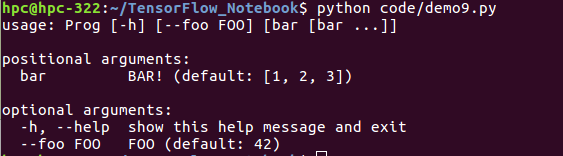
\includegraphics[scale=0.5]{demo8.png}\par
MatavarTypeHelpFormatter用type显示参数显示值的名字。
\begin{python}
import argparse
parser = argparse.ArgumentParser(prog='Prog',
formatter_class = argparse.ArgumentDefaultsHelpFormatter)
parser.add_argument('--foo',type=int,default=42,help='FOO')
parser.add_argument('bar',nargs='*',default=[1,2,3],help='BAR!')
parser.print_help()
\end{python}
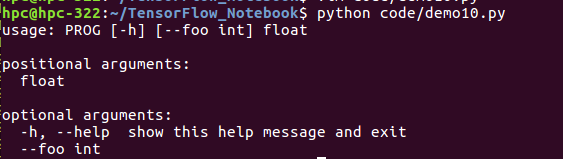
\includegraphics[scale=0.5]{demo9.png}\newline
prefix\_chars,大多数命令行参数选项用-,比如-f/--foo。parsers需要支持不同的或者说另外的前缀,像+f或者/foo
就可以设置prefix\_chars=参数指定。prefix\_chars默认默认为-,用非-字符能禁用-f/--foo这种类型性的选项。\newline
\begin{python}
import argparse
parser = argparse.ArgumentParser(prog='PROG',prefix_chars='-+')
parser.add_argument('+f')
parser.add_argument('++bar')
parser.parse_args('+f X ++bar Y'.split())

\end{python}
fromfile\_prefix\_chars,有时我们处理一个长的参数列表,将参数保存在文件中比直接在命令行中更容易理解,如果fromfile\_prefix\_chars=参数给ArgumentParse结构体,指定的参数将被作为文件,被下面的参数取代。例如
\begin{python}
import argparse
with open('args.txt','w') as fp:
    fp.write('-f\nbar')
parser = argparse.ArgumentParser(fromfile_prefix_chars='@')
parser.add_argument('-f')
parser.parse_args(['-f','foo','@args.txt'])
\end{python}
默认从一个文件读取参数,上面的表达式['-f','foo','@args.txt']等于表达式['-f','foo','-f','bar'],fromfile\_prefix\_chars参数默认为None,意味着参数不被当作文件。
argument\_default\par
通常通过传递add\_argument或者通过调用set\_defaults()方法指定名字和值对,然而有时候通过给参数指定一个简单的parser-wide是有用的,这可以通过传递argument\_default=关键字到ArgumentParser,例如调用其全局抑制属性在parse\_args()调用,我们用argument\_default=SUPPRESS:
\begin{python}
import argparse
parser = argparse.ArgumentParser(argument_default=argparse.SUPPRESS)
parser.add_argument('--foo')
parser.add_argument('bar',nargs='?')
parser.parse_args(['--foo','1','BAR'])
print(parser.parse_args([]))
\end{python}
allow\_abbrev\par
通常我们传递一个参数liebhiao给ArgumentParser的方法parse\_args(),如果选项参数太长的话。特征展示可能通过设置allow\_abbrev设置为False被禁用。
\begin{python}
import argparse
parser = argparse.ArgumentParser(prog='Prog',allow_abbrev=False)
parser.add_argument('--foobar',action='store_true')
parser.add_argument('--fooley',action='store_true')
parser.parse_args(['--foon'])
\end{python}
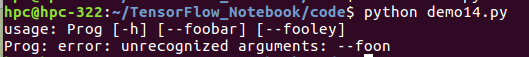
\includegraphics[scale=0.5]{demo10.png}\newline
conflict\_handler\newline
ArgumentParser对象不允许相同的选项字符串有两个行为,默认情况下当已经一偶选项字符串使用时尝试穿件一个新的参数ArgumentParser对象将报出异常。\par
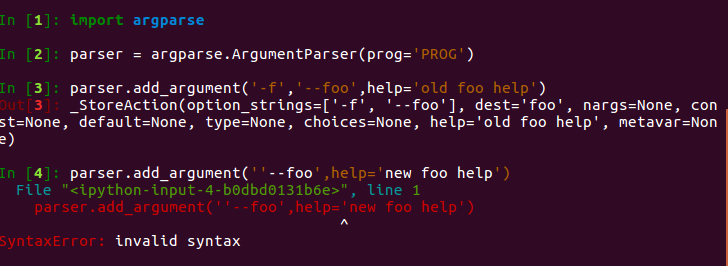
\includegraphics[scale=0.5]{demo11.png}
有时候覆盖掉就得参数时有用的,为了得到参数的行为值'resolcve'可能被应用在conflict\_handler=参数。
\begin{python}
import argparse
parser = argparse.ArgumentParser(prog='PROG',conflict_handler='resolve')
parser.add_argument('-f','--foo',help='old foo help')
parser.add_argument('--foo',help='new foo help')
parser.print_help()
\end{python}

\includegraphics[scale=0.5]{demo12.png}\newline
如果所有的选项字符串被覆盖,ArgumentParser对象仅仅移除一个行为,因此上面的例子中,就得行为-f/--foo行为保留-f行为,因为仅仅--foo选项字符串被覆盖。
add\_help\par
默认情况下ArgumentParserdurian增加帮助信息到显示的消息中,例如:
\begin{python}
import argparse
parser = argparse.ArgumentParser(description='Process some integers.')
parser.add_argument('integers',metavar='N',type=int,nargs='+',help='an integer for the accumulator')
parser.add_argument('--sum',dest='accumulate',action='store_const',const=sum,default=max,help='sum the integers(default:find the max)')
args = parser.parse_args()
print(args.accumulate(args.integers))
\end{python}
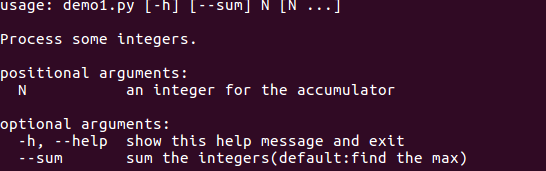
\includegraphics[scale=0.5]{demo13.png}
\begin{python}
import argparse
parser = argparse.ArgumentParser(description='Process some integers.',add_help=False)
parser.add_argument('integers',metavar='N',type=int,nargs='+',help='an integer for the accumulator')
parser.add_argument('--sum',dest='accumulate',action='store_const',const=sum,default=max,help='sum the integers(default:find the max)')
args = parser.parse_args()
print(args.accumulate(args.integers))
\end{python}

\includegraphics[scale=0.5]{demo14.png}
\subsection{add\_argument()方法}
ArgumentParser.add\_argument(name or flags...[, action][, nargs][, const][, default][, type][, choices][, required][, help][, metavar][, dest])
定一个一个命令行参数应该被如何解析,每一个参数自己有自己的详细描述,如下:
\begin{itemize}
\item name or flags:名字或者选项字符串,foo或者(-f,--foo)。
\item action:参数出现在命令行后采取的基本的行为。
\item nargs:命令行参数应该被使用的参数的数量。
\item const:action和nargs选项要求的常数值。
\item default:缺乏参数的默认值。
\item type:传递参数读额数据类型。
\item choices:参数的允许值的容器。
\item required:是否命令行选项被乎略。
\item help:简易的参数说明。
\item metavar:在usage消息的名字。
\item dest:增加到parse\_args()返回对象的属性的名字。
\end{itemize}
name或者flags\par
当parse\_args()被调用的时候。选项参数通过-前缀识别。
\begin{python}
import argparse
parser = argparse.ArgumentParser(prog='PROG')
parser.add_argument('-f','--foo')
parser.add_argument('bar')
print(parser.parse_args(['BAR']))
print(parser.parse_args(['BAR','--foo','FOO']))
\end{python}

\includegraphics[scale=0.5]{demo15.png}
action\par
\begin{itemize}
\item 'store':仅仅保存参数的值,例如
\begin{python}
parser = argparse.ArgumentParser()
parser.add_argument('--foo')
parser.parse_args('--foo 1'.split)
\end{python}
输出Namespace(foo='1')\par
\item 'store\_true':存储const参数指定的值,'store\_const'行为通常用于指定一些flag。
\begin{python}
parser = argparse.ArgumentParser()
parser.add_argument('--foo',action='store_contt',const=42)
parser.add_argument('--foo')
\end{python}
输出:Namescpae(foo=42)
\item 'store\_true'和'store\_false'指定'store\_const'。
\begin{python}
parser = argparse.ArgumentParser()
parser.add_argument('--foo',action='store_true')
parser.add_argument('--bar',action='store_false')
parser.add_argument('--baz',action='store_false')
parser.parse_args('--foo --bar'.split())
\end{python}
输出:Namespace(foo=True,abr=False,baz=True)
\item 'append':一个存储列表,添加每个参数值到列表中,允许选项被多次指定时很有用。
\begin{python}
parser = argparse.ArgumentParser()
parser.add_argument('--str',dest='types',action='append_const',const=str)
parser.add_argument('--int',dest='types',action='append_const',const=int)
parser.parse_args('--str --int'.split())
\end{python}
输出:Namespace(type=[<class 'str'>,<class 'int'>])
\item 'count':关键参数出现的次数。
\begin{python}
parser = argparse.ArgumentParser()
parser.add_argument('--verbose','-v',action='count')
parser.parse_args(['-vvv'])
\end{python}
输出:Namespace(varbose=3)
\item help:打印当前parser所有选项的帮助信息,默认帮助行为被添加到parser。
\item version:add\_argument调用指定version=关键字
\begin{python}
import argparse
parser = argparse.ArgumentParser(prog='PROG')
parser.add_argument('--version',action='versddion',version='(%prog)s 2.0')
parser.parse_args(['--version'])
\end{python}
输出PROG 2.0。
\item 你可以通过传递行为子类或者其它对象的接口传递给action,推荐的方法是扩展Action,覆盖掉\_\_call\_\_方法和\_\_init\_\_。
\begin{python}
class FooAction(argparse.Action):
    def __init__(self,option_strings,dest,nargs=None,**kwargs):
        if nargs is not None:
            raise ValueError("nargs not allowed")
    def __call__(self,parser,namespace,values,option_string=None):
        print('%r%r%r'%(namespace,values,option_string))
        setattr(namespace,self.dest,values)
parser = argparse.ArgumentParser()
parser.add_argument('--foo',action=FooAction)
parser.add_argumentParser('bar',action=FooAction)
args = parser.parse_args('1 -- foo 2'.split)
\end{python}
\end{itemize}
输出:\newline
Namespace(bar=None,foo=None) '1' None\newline
Namespace(bar=1,foo=None) '2' '--foo' \newline
nargs\newline
\begin{itemize}
\item N:一个整数,命令行下的参数被放到一起成为一个列表:
\begin{python}
parser = argparse.ArgumentParser()
parser.add_argument('--foo',nargs=2)
parser.add_argument('bar',nargs=1)
parser.parse_args('c --foo a b'.split())
\end{python}
输出:Namespace(bar=['c'],foo=['a','b'])
\item ?:根据不同情况生成不同的值,如果没有参数指定它的值来自默认生成如果有一个带有-前缀的参数值将被const参数生成,如果指定了值将生成指定值。
\begin{python}
parser = argparse.ArgumentParser()
parser.add_argument('--foo',nargs='?',const='c',default='d')
parser.add_argument('bar',nargs='?',default='d')
parser.parse_args(['XX','--foo','YY'])
parser.parse_args(['XX','--foo'])
parser.parse_args([])
\end{python}
分别输出:\newline
Namespace(bar='XX',foo='YY')\newline
Namespace(bar='XX',foo='x')\newline
Namespace(bar='d',foo='d')\newline
用nargs='?'更常用的用法时允许选项输入输出文件:
\begin{python}
parser = argparse.ArgumentParser()
parser.add_argument('infile',nargs='?',type=argparse.FileType('r'),default=sys.stdin)
parser.add_argument('outfile',nargs='?',type=argparse.FileType('w'),default=sys.stdout)
parser.parse_args(['input.txt','output.txt'])
\end{python}
输出:Namespace(infile=<\_io.TextIOWrapper name='input.txt',encoding='UTF-8'>,
outfile<\_io.TextIOWrapper name='output.txt' encoding='UTF-8'>)
parser.parse\_args([])
输出:
Namespace(infile=<io.TextIOWrapper name='<stdin>' encoding='UTF-8'>,
outfile=<\_io.TextIOWrapper name='<stdout>' encoding='UTF-8'>)
\item *:所有的命令行参数将被放到一个列表中。
\begin{python}
parser = argparse.ArgumentParser()
parser.add_argument('--foo',nargs='*')
parser.add_argument('--bar',nargs='*')
parser.add_argument('--barz',nargs='*')
parser.parse_args('a b --foo x y --bar 1 2'.split())

\end{python}
输出:Namespace(bar=['1','2'],baz=['a','b'],foo=['x','y'])
\item +:所有的命令行参数将被添加到一个列表中,至少需要一个参数肉则将报错。
\begin{python}
parser = argparse.ArgumentParser(prog='PROG')
parser.add_argument('foo',nargs='+')
parser.parse_args(['a','b'])
parser.parse_args([])
\end{python}
输出:Namespace(foo=['a',nargs='+'])\newline
usage: PROG [-h] foo [foo ...]\newline
PROG: error: too few arguments\newline
\item argparse.REMAINDER:所有已经存在的参数被添加到一个列表。
\begin{python}
parser = argparse.ArgumentParser(prog='PROG')
parser.add_argument('--foo')
parser.add_argument('command')
parser.add_argument('args',nargs=argparse.REMAINDER)
print(parser.parse_args('--foo B cmd --arg1 xx zz'.split()))
\end{python}
输出:Namespace(args=['--arg1','XX','ZZ'],command='cmd',foo='B')
如果nargs参数没有提供,argument 由action决定,通常这意味着一个的命令行参数被使用一个项目被产生。
\end{itemize}
const\par
const参数被用在保存没有被命令行读入的常数来常数值,两个常见的用法如下:
\begin{itemize}
\item 当add\_argument()调用的时候设置了action='store\_const'或者是action='append\_cost'通过增加const值到一个parse\_args()返回的对象的属性。
\item 当add\_argument()通过选项字符串(像-f或者--foo)和nargs='?',这将穿件一个由0行或者一行参数跟着的选项,当解析命令行时,如果选项字符串遇到没有命令行参数的时候,值const将被用来替代。'store\_const'和'append\_const'行为,const关键字参数必须给定,对于其它行为,默认为None。
\end{itemize}
default\par
所有的参数和一些位置的参数在命令行下可能被忽略,add\_argument()参数default的值默认为None,指定当没有参数时什么值被使用。没有指定选项字符串,default的值将取代参数。
\begin{python}
parser = argparse.ArgumentParser()
parser.add_argument('--foo',default=42)
parser.parser_args(['--foo','2'])
parser.parse_args([])
\end{python}
输出:
Namespace(foo='2')\newline
Namespace(foo=42)\newline
如果默认值是一个字符串,parser解析值就好象命令行参数一样,类似的,parser应用任何type转换参数,如果在设置属性值前Namespace返回值,否则parser用下面的值。
\begin{python}
parser = argparse.ArgumentParser()
parser.add_argument('--length',default=42,type=int)
parser.add_argument('--width',default=10.5,type=int)
parser.parse_args()
\end{python}
输出:Namesapce(length=10,width=10.5)\newline
对于参数为'?'或者'*',命令行没有值的时候default值将被使用
\begin{python}
parser = argparse.ArgumentParser()
parser.add_argument('foo',nargs='?',default=42)
parser.parse_args(['a'])
parser.parse_args([])
\end{python}
分别输出:\newline
Namespace(foo='a')\newline
Namespace(foo=42)\newline
如果default=argparse.SUPPRESS如果没有命令行参数将导致没有属性被添加。
\begin{python}
parser = argparse.ArgumentParser()
parser.add_argument('--foo',default=argparse.SUPPRESS)
parser.parse_args([])
parser.parse_args(['--foo','1'])
\end{python}
分别输出:\newline
Namespace()\newline
Namespace(foo='1')\newline
type\par
默认ArgumentParser对象读命令行参数为字符串,然而,经常命令行应该以另一种数据类型解析,像float,int,add\_argument()的type关键字允许需要的类型检查和转换被执行,常用的内部数据类型和参数可以被作为type的值直接使用。
\begin{python}
parser = argparse.ArgumentParser()
parser.add_argument('foo',type=int)
parser.add_argument('bar',type=open)
parser.parse_args('2 temp.txt'.split())
\end{python}
输出:Namespace(bar=<\_io.TextIOWrapper name='temp.txt' encoding='UTF-8',foo=2)
为了能轻松的使用多种文件类型,argparse模块提供了工厂FileType,利用mode=,bufsize=,encoding=和error=参数,例如FileType('w')可以被用来创建一个可写的文件。
\begin{python}
parser = argparse.ArgumentParser()
parser.add_argument('bar',type=argparse.FileType('w'))
parser.parse_args(['output'])
\end{python}
输出:Namespace(bar=<\_io.TextIOWrapepr name='out.txt' encoding=;UTF-8;>)
type能够调用一个字符串参数返回转换过值的参数
\begin{python}
import math
import argparse
def perfect_square(string):
    value = int(string)
    sqrt = math.sqrt(value)
    if sqrt!=int(sqrt):
        msg='%r is not a perfect square'%string
        raise argparse.ArgumentTypeError(msg)
    return value
parser = argparse.ArgumentParser(prog='PROG')
parser.add_argument('foo',type=perfect_square)
print(parser.parse_args(['9']))
print(parser.parse_args(['7']))

\end{python}
输出:
Namespace(foo=9)\newline
usage: PROG [-h] foo\newline
PROG: error: argument foo: '7' is not a perfect square\newline
choise\par
choise参数在检查值的范围时很方便。
\begin{python}
parser = argaprse.ArgumentParser(prog='PROG')
parser.add_argument('foo',type=int,choice=range(5,10))
parser.parse_args(['7'])
parser.parse_args(['11'])
\end{python}
分别输出:Namespace(foo=7)\newline
usage: PROG [-h] {5,6,7,8,9}\newline
PROG: error: argument foo: invalid choice: 11 (choose from 5, 6, 7, 8, 9)\newline
choise\par
一些命令行参数从一些限定值的中选定,可以通过传递choice关键字参数给add\_argument(),当命令行解析的时候,值将被检查如果不在可接受值范围内将显示错误消息。
\begin{python}
parser = argparse.ArgumentParser(prof='game.py')
parser.add_argument('move',choices=['rock','paper','scissors'])
parser.parse_args(['rock'])
parser.parse_args(['file'])
\end{python}
分别输出:\newline
Namespace(move='rock')\newline
usage: game.py [-h] {rock,paper,scissors}\newline
game.py: error: argument move: invalid choice: 'fire' (choose from 'rock',
'paper', 'scissors'\newline
choice选项检查在转化数据类型后进行。
\begin{python}
parser = argparse.ArgumentParser(prog='doors.py')
parser.add_argument('door',type=int,choices=range(1,4))
print(parse.parse_args(['3']))
print(parser.parse_args(['4']))
\end{python}
分别输出:\newline
Namespace(door=3)\newline
usage: doors.py [-h] {1,2,3}\newline
doors.py: error: argument door: invalid choice: 4 (choose from 1, 2, 3)\newline
任何支持in操作的对象都能被传递给choise作为值,因此dict,set对象都是常用的支持的对象。
required\par
通常argparse模块假设flag像可以被省略的-f和--bar,,为了一个选项必需要需要设置required=True。
\begin{python}
parser = argparse.ArgumentParser()
parser.add_argument('--foo',required=True)
parser.parse_args(['--foo','BAR'])
parer.parse_args([])
\end{python}
分别输出:\newline
Namespace(foo='BAR')\newline
usage: argparse.py [-h] [--foo FOO]\newline
argparse.py: error: option --foo is required\newline
正如上例,如果parse\_args()的required被标记,如果不给值将报错。
help\par
help值包含一些简单的参数说明,当用户要求帮助的时候(通常用-h或者--help),help描述信息将被展示
\begin{python}
parser = argparse.ArgumentParser(prog='frobble')
parser.add_argument('--foo',action='store_true',help='foo the bars before frobbing')
parser.add_argument('bar',nargs='+',help='foo the bars before frobbed')
parser.parse_args(['-h'])
\end{python}
输出:\newline
usage: frobble [-h] [--foo] bar [bar ...]\newline
positional arguments:\newline
 bar     one of the bars to be frobbled\newline

optional arguments:\newline
 -h, --help  show this help message and exit\newline
 --foo   foo the bars before frobbling\newline
help字符串能包含多种格式像程序名字或者默认参数,可用的指定包含程序的名字,\%(prog)s和多数add\_argument()关键字,像\%(default)s,\%(type)s等等。
\begin{python}
parser = argparse.ArgumentParser(prog='frobble')
parser.add_argument('bar',nargs='?',type=int,default=42,help='the bar to %(prog)s(default:%(default)s)')
parser.print_help()
\end{python}
输出:\newline
usage: frobble [-h] [bar]\newline

positional arguments:\newline
 bar     the bar to frobble (default: 42)\newline

optional arguments:\newline
 -h, --help  show this help message and exit\newline
帮助字符串支持\%格式,如果你想一个\%出现在帮助字符串中,你需要使用\%\%
argparse对于指定的选项通过设置argparse.SUPRESS设置支持静默帮助。
\begin{python}
parser = argaprse.ArgumentParser(prog='frobble')
parser.add_argument('--foo',help=argparse.SUPPRESS)
parse.print_help()
\end{python}
输出:\newline
usage: frobble [-h]\newline

optional arguments:\newline
  -h, --help  show this help message and exit\newline
metavar\par
当ArgumenrParser生成帮助消息的时候需要一些方法设计查询每个参数,默认,ArgumentParser对象用dest值作为每个对象的名字,默认对于action位置的参数,dest值被直接使用,对于一些选项行为,dest值时大写的。因此单个位置参数dest='bar'将被认做bar,--foo应该被跟着一个命令作为FOO
\begin{python}
parser = argparse.ArgumentParser()
parser.add_argument('--foo')
parser.add_argument('bar')
parser.parser_args('X --foo Y'.split())
print.print_help()
\end{python}
分别输出:\newline
Namespace(bar='X',foo='Y')\newline
usage:  [-h] [--foo FOO] bar\newline

positional arguments:\newline
 bar\newline

optional arguments:\newline
 -h, --help  show this help message and exit\newline
 --foo FOO\newline

一个可用的名字被matavar指定:
\begin{python}
parser = argparse.ArgumentParser()
parser.add_argument('--foo',metavar='YYY')
parser.add_argument('bar',metavar='XXX')
parser.parse_args('X -- foo Y'.split())
parser.print_help()
\end{python}
Namespace(abr='X',foo='Y')\newline
usage:  [-h] [--foo YYY] XXX\newline

positional arguments:\newline
 XXX\newline

optional arguments:\newline
 -h, --help  show this help message and exit\newline
 --foo YYY\newline
注意matavar仅仅改变显示的名字,parse\_args()属性的名字仍然由dest值决定。不同的nargs也许导致metavar被多次使用,提供一个元组给metavar指定一个不同的显示。
\begin{python}
parser = argparse.ArgumentParser(prog='prog')
parser.add_argument('-x',nargs=2)
parser.add_argument('--foo',nargs=2,metavar=('bar','baz'))
parser.print_help()
\end{python}
输出:\newline
usage: PROG [-h] [-x X X] [--foo bar baz]\newline

optional arguments:\newline
 -h, --help     show this help message and exit\newline
 -x X X\newline
 --foo bar baz\newline
dest\par
大多数ArgumentPArser行为增加一些值作为parser\_args()返回值的属性。属性的名字由dest决定
\begin{python}
parser = argparse.ArgumentParser()
parser.add_argument('bar')
parser.parse_args(['xxx'])
\end{python}
输出:Namespace(bar='xxx')\newline
对于选项参数,dest的值从选项字符串推断出,ArgumentParser通过得到长的选项字符串删除初始化--字符串生成dest的值,如果meiyoiu长的选项字符串提供,dest将通过初始化字符-从第一个短的字符串选项得到。任何内部-字符将被转换为\_字符确保字符串是一个可用的属性名字。
\begin{python}
parser = argparse.ArgumentParser()
parser.add_argument('-f','--foo-bar','--foo')
parser.add_argument('-x','-y')
parser.parse_args('-f 1 -x 2'.split())
parser.parse_args('--foo 1 -y 2'.split())
\end{python}
分别输出:\newline
Namespace(foo\_bar=1,x='2')\newline
Namespace(foo\_bar='1',x='2')\newline
dest允许自定义属性的名字:
\begin{python}
parser = argparse.ArgumentParser()
parser.add_argument('--foo',dest='bar')
parser.parse_args('--foo XXX'.split())
\end{python}
输出:Namespace(bar='XXX')\newline
Action class\par
Action classes 实现的Action API,一个命令行返回的可调的API。任何这个API对象都可以被zuoiweiaction参数传递给add\_argument()。
class argparse.Action(option\_strings, dest, nargs=None, const=None, default=None, type=None, choices=None, required=False, help=None, metavar=None)
Action实力应该是可调用的,因此子类必须被\_\_call\_\_方法覆盖,应该接受四个参数:
\begin{itemize}
\item parser:包含这个action的ArgumentParser。
\item namespace:parser\_args()返回的Namespace对象,大多数行为通过setattr()增加一个属性到对象。
\item varlue:结合命令行参数和任何转化应用,类型转换被type关键字指定。
\item option\_string:宣告像字符串被用于激活这个action,option\_string时一个选项,将缺席如果这个action和positional参数结合。
\_\_call\_\_方法也许执行任意行为,但是典型的设置基于dest和value的namespace属性。
\end{itemize}
parse\_args()方法:\par
ArgumentParser.parse\_args(args=None, namespace=None)
转换参数字符串为对象指定他们作为namespace的属性。之前调用add\_argument()决定
决定创建什么对象如何复制,默认argument字符串来自sys.argv,一个新的空的Namespace对象被创建。
Option value syntax\par
parse\_args方法支持多种方法指定选项的值,在最简单的情况下,这个选项和它的值被传递作为两个分开的参数:
\begin{python}
parser = argparse.ArgumentParser(prog='PROG')
parser.add_argument('-x')
parser.add_argument('--foo')
parser.parse_argument('-x','X')
parser.parse_args('--foo','FOO')
\end{python}
分别输出:\newline
Namespace(foo=None,x='X')\newline
Namespace(foo='FOO',x=None)\newline
对于短的选项,这个选项值可以被链接,多个短选项可以被-前缀连接在一起,只要最新的选项(非空)要求值:
\begin{python}
parser = argparse.ArgumentParser(prog='PROG')
parser.add_argument('-x',action='store_true')
parser.add_argument('-y',action='store_true')
parser.add_argument('-z')
parser.parse_args(['-xyzZ'])
\end{python}
输出:Namespace(x=True,y=True,z='Z')
不可用的参数\par
当解析命令行时parse\_args()检查多种错误,包括不明确的选项,不可用的类型,错误的参数为值等等,当出现一个错误,它推出同时打印错误和用法信息。
\begin{python}
parser = argparse.ArgumentParser(prog='PROG')
parser.add_argument('--foo', type=int)
parser.add_argument('bar', nargs='?')

# invalid type
parser.parse_args(['--foo', 'spam'])
usage: PROG [-h] [--foo FOO] [bar]
PROG: error: argument --foo: invalid int value: 'spam'

# invalid option
parser.parse_args(['--bar'])
usage: PROG [-h] [--foo FOO] [bar]
PROG: error: no such option: --bar

# wrong number of arguments
parser.parse_args(['spam', 'badger'])
usage: PROG [-h] [--foo FOO] [bar]
PROG: error: extra arguments found: badger
\end{python}
参数包含\par
当用户犯错时parse\_args()方法尝试给出错误,但是一些情况下固有的二义,例如,命令行参数-1可能苍时指定一个选项或者尝试提供一个指定位置参数,parse\_args()方法导致,指定位置的参数仅仅用-开始如果他们看起来像负数在parser没有选像解析看起来像负数:
\begin{python}
parser = argparse.ArgumentParser(prog='PROG')
parser.add_argument('-x')
parser.add_argument('foo', nargs='?')

# no negative number options, so -1 is a positional argument
parser.parse_args(['-x', '-1'])
Namespace(foo=None, x='-1')

# no negative number options, so -1 and -5 are positional arguments
parser.parse_args(['-x', '-1', '-5'])
Namespace(foo='-5', x='-1')

parser = argparse.ArgumentParser(prog='PROG')
parser.add_argument('-1', dest='one')
parser.add_argument('foo', nargs='?')

# negative number options present, so -1 is an option
parser.parse_args(['-1', 'X'])
Namespace(foo=None, one='X')

# negative number options present, so -2 is an option
parser.parse_args(['-2'])
usage: PROG [-h] [-1 ONE] [foo]
PROG: error: no such option: -2

# negative number options present, so both -1s are options
parser.parse_args(['-1', '-1'])
usage: PROG [-h] [-1 ONE] [foo]
PROG: error: argument -1: expected one argument
\end{python}
如果你有一个必须以-开始的参数而且不是负数,你可以插入'--'告诉parse\_args()之后的一切:
\begin{python}
parser.parse_args(['--','-f'])
\end{python}
输出:Namespace(foo='-f',one=None)
参数缩略
如果缩略没有歧义parser\_args()方法默认允许长选项被简写为前缀.
\begin{python}
parser = argparse.ArgumentParser(prog='PROG')
parser.add_argument('-bacon')
parser.add_argument('-badger')
parser.parse_args('-bac MMM'.split())
Namespace(bacon='MMM', badger=None)
arser.parse_args('-bad WOOD'.split())
Namespace(bacon=None, badger='WOOD')
arser.parse_args('-ba BA'.split())
usage: PROG [-h] [-bacon BACON] [-badger BADGER]
PROG: error: ambiguous option: -ba could match -badger, -bacon
\end{python}
可能产生多个选项时错误产生,可以通过设置allow\_abbrev设置为False禁用。
Beyond sys.args\par
ArgumentParser通常比sys.argv有用,可以穿地一个字符串列表到parser\_args()完成,这在测试交互式提示符很有用。
\begin{python}
parser = argparse.ArgumentParser()
parser.add_argument('integers',metavar='int',type=int,choice=range(100),
nargs='+',help='an integer in range 0..9')
parser.add_argument('--sum',dest='accumulate',action='store_const',
const=sum,default=max,help='sum the integers (default:find the max)')
parser.parse_args(['1','2','3','4'])
parser.parse_args(['1','2','3','4'],'--sum')
\end{python}
输出结果分别为:\newline
Namespace(accumulate=<built-in function max>,integers=[1,2,3,4])\newline
Namespace(accumulate=<built-in function sum>,integers=[1,2,3,4])\newline
Namespace对象\par
class argparse.Namespace,简单的parse\_args()创建一个对象,保存属性返回它。
这个类很简单,仅仅是一个可读表达的对象子类,如果你希望有字典类似的属性,你可以用标准的python idiom():
\begin{python}
parser = argparse.ArgumentParser()
parser.add_argument('--foo')
args = parser.parse_args(['--foo','BAR'])
var(args)
\end{python}
输出{'foo':'BAR'}\newline
当ArgumentParser指定属性到已经存在的对象时它是很有用的,相比于新的Namespaced对象,它可以指定namespace=关键参数获得。
\begin{python}
class C:
    pass
C = C()
parser = argparse.ArgumentParser()
parser.add_argument('--foo')
parser.parse_args(args=['--foo','BAR'],namespace=C)
c.foo
\end{python}
输出:'BAR'\newline
子命令:
ArgumentParser.add\_subparsers([title][, description][, prog][, parser\_class][, action][, option\_string][, dest][, help][, metavar])
一些程序分割他们的功能为一个子命令,例如,svn程序可以有子命令svn checkout,svn commit,svn update。当程序有一些要求不同类型命令行参数的不同的功能的时候分割功能的方法是一个好的想法,ArgumentParser支持支持add\_subparsers一个子命令,add\_subparsers()方法调用通常没有参数返回一个特殊的行为对象,这个对象是一个方法,add\_parser()得到一个命令名字和任何ArgumentParser够草体参数,返回一个可以被修改的ArgumentParser对象。
\begin{itemize}
\item title:帮助输出sub-parser组的标题,如果说明提供了的话默认"subcommands",否则用参数作为标题。
\item description:在输出帮助中描述sub-parser组,默认是None。
\item prog:sub-command的帮助信息,默认程序的名字和位置上的参数在subparser参数前。
\item parser\_class:用于创建一个sub-parser实例的类,默认时当parser。
\item action:在命令行中参数出现厚的基础类型的行为。
\item dest:sub-command下属性的名字将被存储,默认没有值被存储。
\item help:在帮助输出的sub-parser,默认为None。
\item matavar:在help中可用的子命令默认是None代表子命令{cmd1,cmd2,\dots}
\end{itemize}
用法:
\begin{python}
# create the top-level parser
parser = argparse.ArgumentParser(prog='PROG')
parser.add_argument('--foo', action='store_true', help='foo help')
subparsers = parser.add_subparsers(help='sub-command help')

# create the parser for the "a" command
parser_a = subparsers.add_parser('a', help='a help')
parser_a.add_argument('bar', type=int, help='bar help')

# create the parser for the "b" command
parser_b = subparsers.add_parser('b', help='b help')
parser_b.add_argument('--baz', choices='XYZ', help='baz help')

# parse some argument lists
parser.parse_args(['a', '12'])
Namespace(bar=12, foo=False)
parser.parse_args(['--foo', 'b', '--baz', 'Z'])
Namespace(baz='Z', foo=True)
\end{python}
注意parser\_args()返回的durian将包含住parser和subparser命令行选中的参数,因此在上面的例子中,当一个命令被指定,仅仅foo和bar被呈现,当b被指定,仅仅foo和baz属性被呈现,类似的,subparser要求帮助信息,仅仅这个parser的帮助信息被打印,帮助信息不包含父或者兄弟parser信息。(一个subparser命令的帮助消息,然而,可以被help=参数增加到上面)
\begin{python}
parser.parse_args(['--help'])
usage: PROG [-h] [--foo] {a,b} ...

positional arguments:
  {a,b}   sub-command help
    a     a help
    b     b help

optional arguments:
  -h, --help  show this help message and exit
  --foo   foo help

parser.parse_args(['a', '--help'])
usage: PROG a [-h] bar

positional arguments:
  bar     bar help

optional arguments:
  -h, --help  show this help message and exit

parser.parse_args(['b', '--help'])
usage: PROG b [-h] [--baz {X,Y,Z}]

optional arguments:
  -h, --help     show this help message and exit
  --baz {X,Y,Z}  baz help 
\end{python}
add\_subparsers()方法也支持title和discription关键参数,当两者都呈现的时候在帮助输出subparser的命令将出现在自己的组。
\begin{python}
>>> parser = argparse.ArgumentParser()
>>> subparsers = parser.add_subparsers(title='subcommands',
...                                    description='valid subcommands',
...                                    help='additional help')
>>> subparsers.add_parser('foo')
>>> subparsers.add_parser('bar')
>>> parser.parse_args(['-h'])
usage:  [-h] {foo,bar} ...

optional arguments:
  -h, --help  show this help message and exit

subcommands:
  valid subcommands

  {foo,bar}   additional help
\end{python}
更进一步,add\_parser支持一个aliases参数,允许多字符串访问同一个subparser,像svm,别名co作为checkout的简写。
\begin{python}
>>> parser = argparse.ArgumentParser()
>>> subparsers = parser.add_subparsers()
>>> checkout = subparsers.add_parser('checkout', aliases=['co'])
>>> checkout.add_argument('foo')
>>> parser.parse_args(['co', 'bar'])
Namespace(foo='bar')
\end{python}
一个类似的高效处理sub-commands结合add\_subparsers()方法调用set\_default()以至于每个subparser知道那个python函数应该被执行。
\begin{python}
>>> # sub-command functions
>>> def foo(args):
...     print(args.x * args.y)
...
>>> def bar(args):
...     print('((%s))' % args.z)
...
>>> # create the top-level parser
>>> parser = argparse.ArgumentParser()
>>> subparsers = parser.add_subparsers()
>>>
>>> # create the parser for the "foo" command
>>> parser_foo = subparsers.add_parser('foo')
>>> parser_foo.add_argument('-x', type=int, default=1)
>>> parser_foo.add_argument('y', type=float)
>>> parser_foo.set_defaults(func=foo)
>>>
>>> # create the parser for the "bar" command
>>> parser_bar = subparsers.add_parser('bar')
>>> parser_bar.add_argument('z')
>>> parser_bar.set_defaults(func=bar)
>>>
>>> # parse the args and call whatever function was selected
>>> args = parser.parse_args('foo 1 -x 2'.split())
>>> args.func(args)
2.0
>>>
>>> # parse the args and call whatever function was selected
>>> args = parser.parse_args('bar XYZYX'.split())
>>> args.func(args)
((XYZYX))
\end{python}
你可以用parse\_args()在参数解析完成后通过调用合适的函数做这个工作,结合函数和action像这个像这样典型的轻松的方法处理不同的行为,然而,如果它需要检查subparse的名字,dest关键值通过add\_argparsers()调用将发挥作用。
\begin{python}
>>> parser = argparse.ArgumentParser()
>>> subparsers = parser.add_subparsers(dest='subparser_name')
>>> subparser1 = subparsers.add_parser('1')
>>> subparser1.add_argument('-x')
>>> subparser2 = subparsers.add_parser('2')
>>> subparser2.add_argument('y')
>>> parser.parse_args(['2', 'frobble'])
Namespace(subparser_name='2', y='frobble')
\end{python}
FileTyp对象:\newline
class argparse.FileType(mode='r', bufsize=-1, encoding=None, errors=None)
FileType工厂创建一个能被传递给ArgumentParser.add\_argument()的对象。参数有FileType对象将用要求的模式打开命令行参数作为文件,换从大小,编码,错误处理。
\begin{python}
parser = argparser.ArgumentParser()
parser.add_argument('--raw',type=argparse.FileType('wb',0))
parser.add_argument('out'mtype=argparse.FileType('w',encoding='UTF-8'))
parser.parse_args(['--raw','raw.dat','file.txt'])
\end{python}
输出:Namespace(out<\_io.TextIOWapper name='file.txt' mode='w' encoding='UTF-8',raw=<\_ioFileIO name='raw.dat' mode='wb'>)\par
FileType对象明白伪参数同时自动转换sys.stdin为可读的FileType对象,sys.stdout
可写的FileType对象。
\begin{python}
parser = argparse.ArgumentParser()
parser.add_argument('infile',type=argparse.FileType('r'))
parser.parse_args(['-'])
\end{python}
输出Namespace(infile<\_io.TextIOWrapper name='<stdin>' encoding='UTF-8')
Argument group\newline
ArgumentParser.add\_argument\_group(title=None, description=None)\newline
默认情况下,ArgumentParser groups,当显示帮助信息的时候命令行参数进入对应位置的参数和选项参数。当有一个比默认更好的概念上的参数组,合适的组能被add\_argument\_group()创建:
\begin{python}
parser = argparse.ArgumentParser(prog='PROG',add_help=False)
group = parser.add_argument_group('group')
group.add_argument('--foo',help='foo help')
group.add_argument('bar',help='bar help')
parser.print_help()

\end{python}
输出:
usage: PROG [--foo FOO] bar\newline

group:\newline
  bar    bar help\newline
  --foo FOO  foo help\newline
add\_argument\_group()方法返回一个有add\_argument()方法的参数组对象。当一个参数增加到组中,parser就当它为正常参数,但是在帮助信息中分组显示。add\_argument\_group()方法接受title和description参数自定义显示:
\begin{python}
parser = argparse.ArgumentParser(prog='PROG',add_help=False)
group1 = parser.add_argument_group('group1','group1 description')
group1.add_argument('foo',help='foo help')
group2 = parser.add_argument_group('group2','group2 description')
group2.add_argument('--bar',help='bar help')
parser.print_help()
\end{python}
usage: PROG [--bar BAR] foo\newline

group1:\newline
  group1 description\newline

  foo    foo help\newline

group2:\newline
  group2 description\newline

  --bar BAR  bar help\newline
注意任何不再你的用户定义组中的参数将以对应位置参数和选项参数结束。
Mutual exclusion\par
ArgumentParser.add\_mutually\_exclusive\_group(required=False)\par
创建一个转悠的组,argparse将确保惟一的参数在彼此的组被呈现在命令行。
\begin{python}
parser = argparse.ArgumentParser(prog='PROG')
group = parser.add_mutually_exclusive_group()
groud.add_argument('--foo',action='store_true')
groud.add_argument('--bar',action='store_false')
parser.parse_args(['--foo'])
parser.parse_args(['--bar'])
parser.parse_args(['--foo','--bar'])
\end{python}
分别输出:\newline
Namespace(bar=True,foo=True)\newline
Namespace(bar=False,foo=False)\newline
sage: PROG [-h] [--foo | --bar]\newline
PROG: error: argument --bar: not allowed with argument --foo\newline
add\_mutually\_exclusive\_group()方法接受一个required参数,预示着最新的参数被要求。
\begin{python}
parser = argparse.ArgumentParser(prog='PROG')
group = parser.add_mutually_exclusive_group(required=True)
group.add_argument('--foo',action='store_true')
group.add_argument('--bar',action='store_true')
parser.parse_args([])
\end{python}
输出:\newline
usage: PROG [-h] (--foo | --bar)\newline
PROG: error: one of the arguments --foo --bar is required\newline
注意当前的mutually exclusive 参数组不支持title和description参数。
Parser defaults\par
ArgumentParser.set\_defaults(**kwargs)\newline
大多数时候,parse\_args()返回的属性对象将被命令行参数和参数行为完全决定。set\_default()允许一些额外的属性决定没有命令行增加时的行为:
\begin{python}
parser = argparse.ArgumentParser()
parser.add_argument('foo',type=int)
parser.set_default(bar=42,baz='badger')
parser.parse_args(['736'])
\end{python}
输出:Namespace(bar=42,baz='badger',fpp=736)
注意parser级默认覆盖参数级。
\begin{python}
parser = argparser.ArgumentParser()
parser.add_argument('--foo',default='bar')
parser.set_defaults(foo='spam')
parser.parse_args([])
\end{python}
输出:
Namespace(foo='spam')
Parser级别在多个parser时特别有用。
ArgumentParser.get\_default(dest)
得到namespace属性的默认值,正如设置add\_argument()或者set\_defaults()
\begin{python}
parser = argparse.ArgumentParser()
parser.add_argument('--foo',default='badger')
parser.get_default('foo')
\end{python}
输出:'baadger'
Printing help\par
在一些典型的应用中parse\_args()将考虑打印用法和错误信息的格式,然而一些格式方法是可用的:
ArgumentParser.print\_usage(file=None):打印ArgumentParser应该在命令行调用的简单描述,如果file是None,sys.stdout被假定。
ArgumentParser.print\_help(file=None):打印程序的用法信息和ArgumentParser参数注册信息,如果fike时None,sys.stdout被假定。
ArgumentParser.format\_usage():返回在命令行中ArgumentParser参数应该被如何调用的简要说明字符串。
ArgummentParser.format\_help():返回一个包含程序用法和ArgumentParser参数注册信息的帮助字符串。
Partial parsing\par
ArgumentParser.parse\_known\_args(args=None, namespace=None)\newline
有时候一些脚本也许仅仅解析一些命令行参数,传递参数到另一个脚本或者程序,在这种情形下,parser\_know\_args()方法很有用,它像parser\_args()除了当有额外的参数呈现的时候不生成错误,相反,它返回一个包含populated namespace和保留参数字符串的列表的两个元素的元组。
\begin{python}
parser = argparse.ArgumentParser()
parser.add_argument('--foo',action='store_true')
parser.add_argument('bar')
parser.parse_know_args(['--foo','--badger','BAR','spam'])
\end{python}
输出:(Namespace(bar='BAR', foo=True), ['--badger', 'spam'])
Customizing file parsing\par
ArgumentParser.convert\_arg\_line\_to\_args(arg\_line)\newline
从文件中读入的参数一行读一个,convert\_arg\_line\_to\_args()能被覆盖。这个方法从参数文件得到一个简单的arg\_line字符串,返回一个参数列表,每读取一行方法被调用一次。一个有用的覆盖每这个方法是当空格分开的word为参数,下面的例子展示:
\begin{python}
class NyArgumentParser(argparse.ArgumentParser):
    def convert_tag_line_to_args(self,arg_line):
        return arg\_line.split()
\end{python}
Exiting method\par
ArgumentParser.exit(status=0, message=None):这个方法终止程序,以指定的状态推出,如果参数被给,打印消息。
ArgumentParser.error(message):这个方法打印包含消息用法信息到标准错误终止程序以状态代码2。
Upgrading optparse code\par
最初argparse模块尝试用optparse维持兼容性,然而optparse很难扩展,特别是改变要求支持新的nargs=指定更好的用法消息。当大多数optparse已经被复制粘贴过或者monkey-patched,它不再尝试维持向后兼容。,argparse模块在一些方法改进了标准库optparse:
\begin{itemize}
\item 处理位置参数。
\item 支持子命令。
\item 允许+和/前缀。
\item 处理0或者更多1或者更多风格的参数。
\item 处理更多的用法消息。
\item 提供简单的接口自定义type和action。
\end{itemize}
optparse到argparse的并行升级
\begin{python}
\item 用ArgumentParser.add_argument()调用取代optparse.OptionParser.add_option()调用。
\item 用args=parser.parser_args()取代(options,args)=parser.parse_args()增加ArgumentParser.add_argument()调用给指定位置的参数,记住显现的前向,现在在argparse上下文称为args。
\item 用type和action取代callback行为和callback\_*关键参数。
\item 取代type关键字的字符串名字和相关的对象类型(如int,float,complex等等)
\item 用Namespace和optparse.OptionError,optparse.OptionValueError取代optparse.Value。
\item 用标准那得Python语法取代\%default或者\%prog,\%(default)s和\%(prog)s。
\item 通过调用parser.add\_argument('--version',action='version',version='<the version>')取代OptionParser结构体version。
\end{python}
setting
输入:\newline
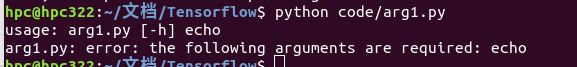
\includegraphics[scale=0.5]{arg1.png}\newline
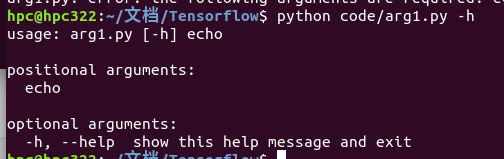
\includegraphics[scale=0.5]{arg2.png}\newline
add\_argument方法指定程序需要接受的命令参数,本例中为echo,此程序运行必须指定一个参数,方法parse\_args()通过分析指定的参数返回数据echo。
\begin{python}
import argparse
parser = argparse.ArgumentParser()
parser.add_argument("echo",help="show the help information",type=int)
args = parser.parse_args()
print(args.echo**2)
\end{python}
指定参数类型为int,默认为string。
\begin{python}
import argparse
parser = argparse.ArgumentParser()
parser.add_argument("--verbosity",help="increase output verbosity")
args = parser.parse_args()
if args.verbosity:
    print("Verbosity turned on")
\end{python}

\includegraphics[scale=0.5]{arg3.png}\newline
这里指定了--verbosity程序就显示一些信息,如果不指定程序也不会出错,对应的变量就被设置为None。
\begin{python}
import argparse
parser = argparse.ArgumentParser()
parser.add_argument("--verbosity",help="increase output verbosity",action="store_true")
args = parser.parse_args()
if args.verbosity:
    print("Verbosity turned on")
\end{python}
指定一个新的关键词action,赋值为store\_ture。如果指定了可选参数,args.verbose就赋值为True,否则就为False。
\begin{python}
import argparse
parser = argparse.ArgumentParser()
parser.add_argument("-v","--verbose",help="Increase output verbosity",action="store_true")
args = parser.parse_args()
if args.verbose:
    print("verbosity turned on")
\end{python}
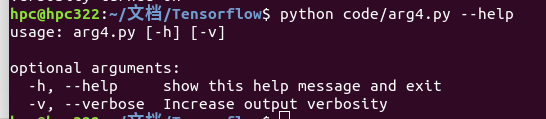
\includegraphics[scale=0.5]{arg4.png}\newline
\begin{python}
#args5.py
import argparse
parser = argparse.ArgumentParser()
parser.add_argument("square",type=int,help="display help information")
parser.add_argument("-v","--verbose",action="store_true",help="increase output verbosity")
args = parser.parse_args()
answer = args.square**2
if args.verbose:
    print("The square of {} equals {}".format(args.square,answer))
else:
    print(answer)
\end{python}
输入参数--verbose和整数(4)顺序不影响结果。
python args5.py --verbose 4和python args5.py 4 --verbose
\begin{python}
import argparse
parser = argparse.ArgumentParser()
parser.add_argument("square",type=int,help="display a square of a given number")
parser.add_argument("-v","--verbosity",type=int,help="increase output verbosity")
args = parser.parse_args()
answer = args.square**2
if args.verbosity == 2:
    print("The square of {} equals {}".format(args.square,answer))
elif args.verbosity == 1:
    print("{}^2=={}".format(args.square,answer))
else:
    print(answer)
\end{python}
python args6.py 4 -v 0,1,2通过指定不同的参数v为0,1,2得到不同的结果。
\begin{python}
#arg7.py
import argparse
parser = argparse.ArgumentParser()
parser.add_argument("square",type=int,help="display the square of a given number")
parser.add_argument("-v","--verbosity",action="count",help="increase output verbosity")
args = parser.parse_args()
answer = args.square**2
if args.verbosity == 2:
    print("The square of {} equals {}".format(args.square,answer))
elif args.verbosity == 1:
    print("{}^2 == {}".format(args.square,answer))
else:
    print(answer)
\end{python}
这里添加参数action="count",统计可选参数出现的次数。
python arg7.py 4 -v(出现一次),对应结果为x\^{}2 == 16\newline
python arg7.py 4 -vv(出现两次),对应出现The square of 4 equals 16\newline
\begin{python}
import argparse
parser = argparse.ArgumentParser()
parser.add_argument("square",type=int,help="display a square of a given number")
parser.add_argument("-v","--verbosity",action="count",default = 0,help="increase output verbosity")
args = parser.parse_args()
answer = args.square**2
if args.verbosity>=2:
    print("The square of {} equals {}".format(args.square,answer))
elif args.verbosity>=1:
    print("{}^2 == {}".format(args.square,answer))
else:
    print(answer)
\end{python}
加速让default参数。这只默认为值0,当参数v不指定时参数就被置为None,None不能和整型比较。
\begin{python}
import argparse
parser = argparse.ArgumentParser()
parser.add_argument("x",type=int,help="The base")
parser.add_argument("y",type=int,help="The exponent")
parser.add_argument("-v","--verbosity",action="count",default=0)
args = parser.parse_args()
answer = args.x**args.y
if args.verbosity >=2:
    print("{} to the power {} equals {}".format(args.x,args.y,answer))
elif args.verbosity >=1:
    print("{}^{} == {}".format(args.x,args.y,answer))
else:
    print(answer)
\end{python}
为了让后面的参数不冲突,我们需要使用另一个方法:
\begin{python}
#args10.py
import argparse
parser = argparse.ArgumentParser()
group = parser.add_mutually_exclusive_group()
parser.add_argument("-v","--verbose",action="store_true")
group.add_argument("-q","--quit",action="store_true")
parser.add_argument("x",type=int,help="The base")
parser.add_argument("y",type=int,help="The exponent")
args = parser.parse_args()
answer = args.x**args.y
if args.quit:
    print(answer)
elif args.verbose:
    print("{} to the power {} equals {}".format(args.x,args.y,answer))
else:
    print("{}^{} == {}".format(args.x,args.y,answer))
\end{python}
可以输入python arg10.py 3 4 -vq得到计算结果。
\begin{python}
import argparse
parser = argparse.ArgumentParser()
group = parser.add_mutually_exclusive_group()
group.add_argument("-v","--verbose",action="store_true")
group.add_argument("-q","--quit",action="store_true")
parser.add_argument("x",type=int,help="The sase")
parser.add_argument("y",type=int,help="The exponent")
args = parser.parse_args()
answer = args.x**args.y
if args.quit:
    print(answer)
elif args.verbose:
    print("{} to the power {} equals {}".format(args.x,args.y,answer))
else:
    print("{}^{} == {}".format(args.x,args.y,answer))
\end{python}
这里参数v和q不能同时使用。

